\documentclass[11pt a4paper]{article}
\usepackage[margin=2cm]{geometry}
\usepackage{amsmath, amssymb}
\usepackage{graphicx}
\usepackage{float}
\usepackage{aligned-overset}
\usepackage{subcaption}

% partielle ableitungen
\newcommand{\delr}{\partial_r}
\newcommand{\deltheta}{\partial_\theta}
\newcommand{\delphi}{\partial_\varphi}

% elektrische feldkonstante
\newcommand{\epsz}{\epsilon_0}
% 1 / 4pi eps
\newcommand{\kco}{\frac{1}{4\pi\epsilon_0}}

% rotation
\newcommand{\rot}{\text{rot}}

% fancy header
\usepackage{fancyhdr}
\fancyhf{}
% vspaces in den headern fuer Distanzen notwendig
% linke Seite: Namen der Abgabegruppe
\lhead{\textbf{Matthias Maile\\Roman Surma}\vspace{1.5cm}}
% rechte Seite: Modul, Gruppe, Semester
\rhead{\textbf{Physik II - Gruppe 2\\Sommersemester 2020}\vspace{1.5cm}}
% Center: nr. des blattes
\chead{\vspace{2.5cm}\huge{\textbf{18. Übungsblatt}}}
% benoetigt damit der eigentliche Text nicht in der Überschrift steckt
\setlength{\headheight}{4cm}

% zum zeichnen tikz
\usepackage{tikz}

% fuer fabigen text
\usepackage{xcolor}

% irgendwas mit figures
\usepackage{subcaption}

\begin{document}
\thispagestyle{fancy}
\section*{Aufgabe 1}
a)
\begin{figure}[H]
	\centering
	\begin{subfigure}[b]{0.3\textwidth}
		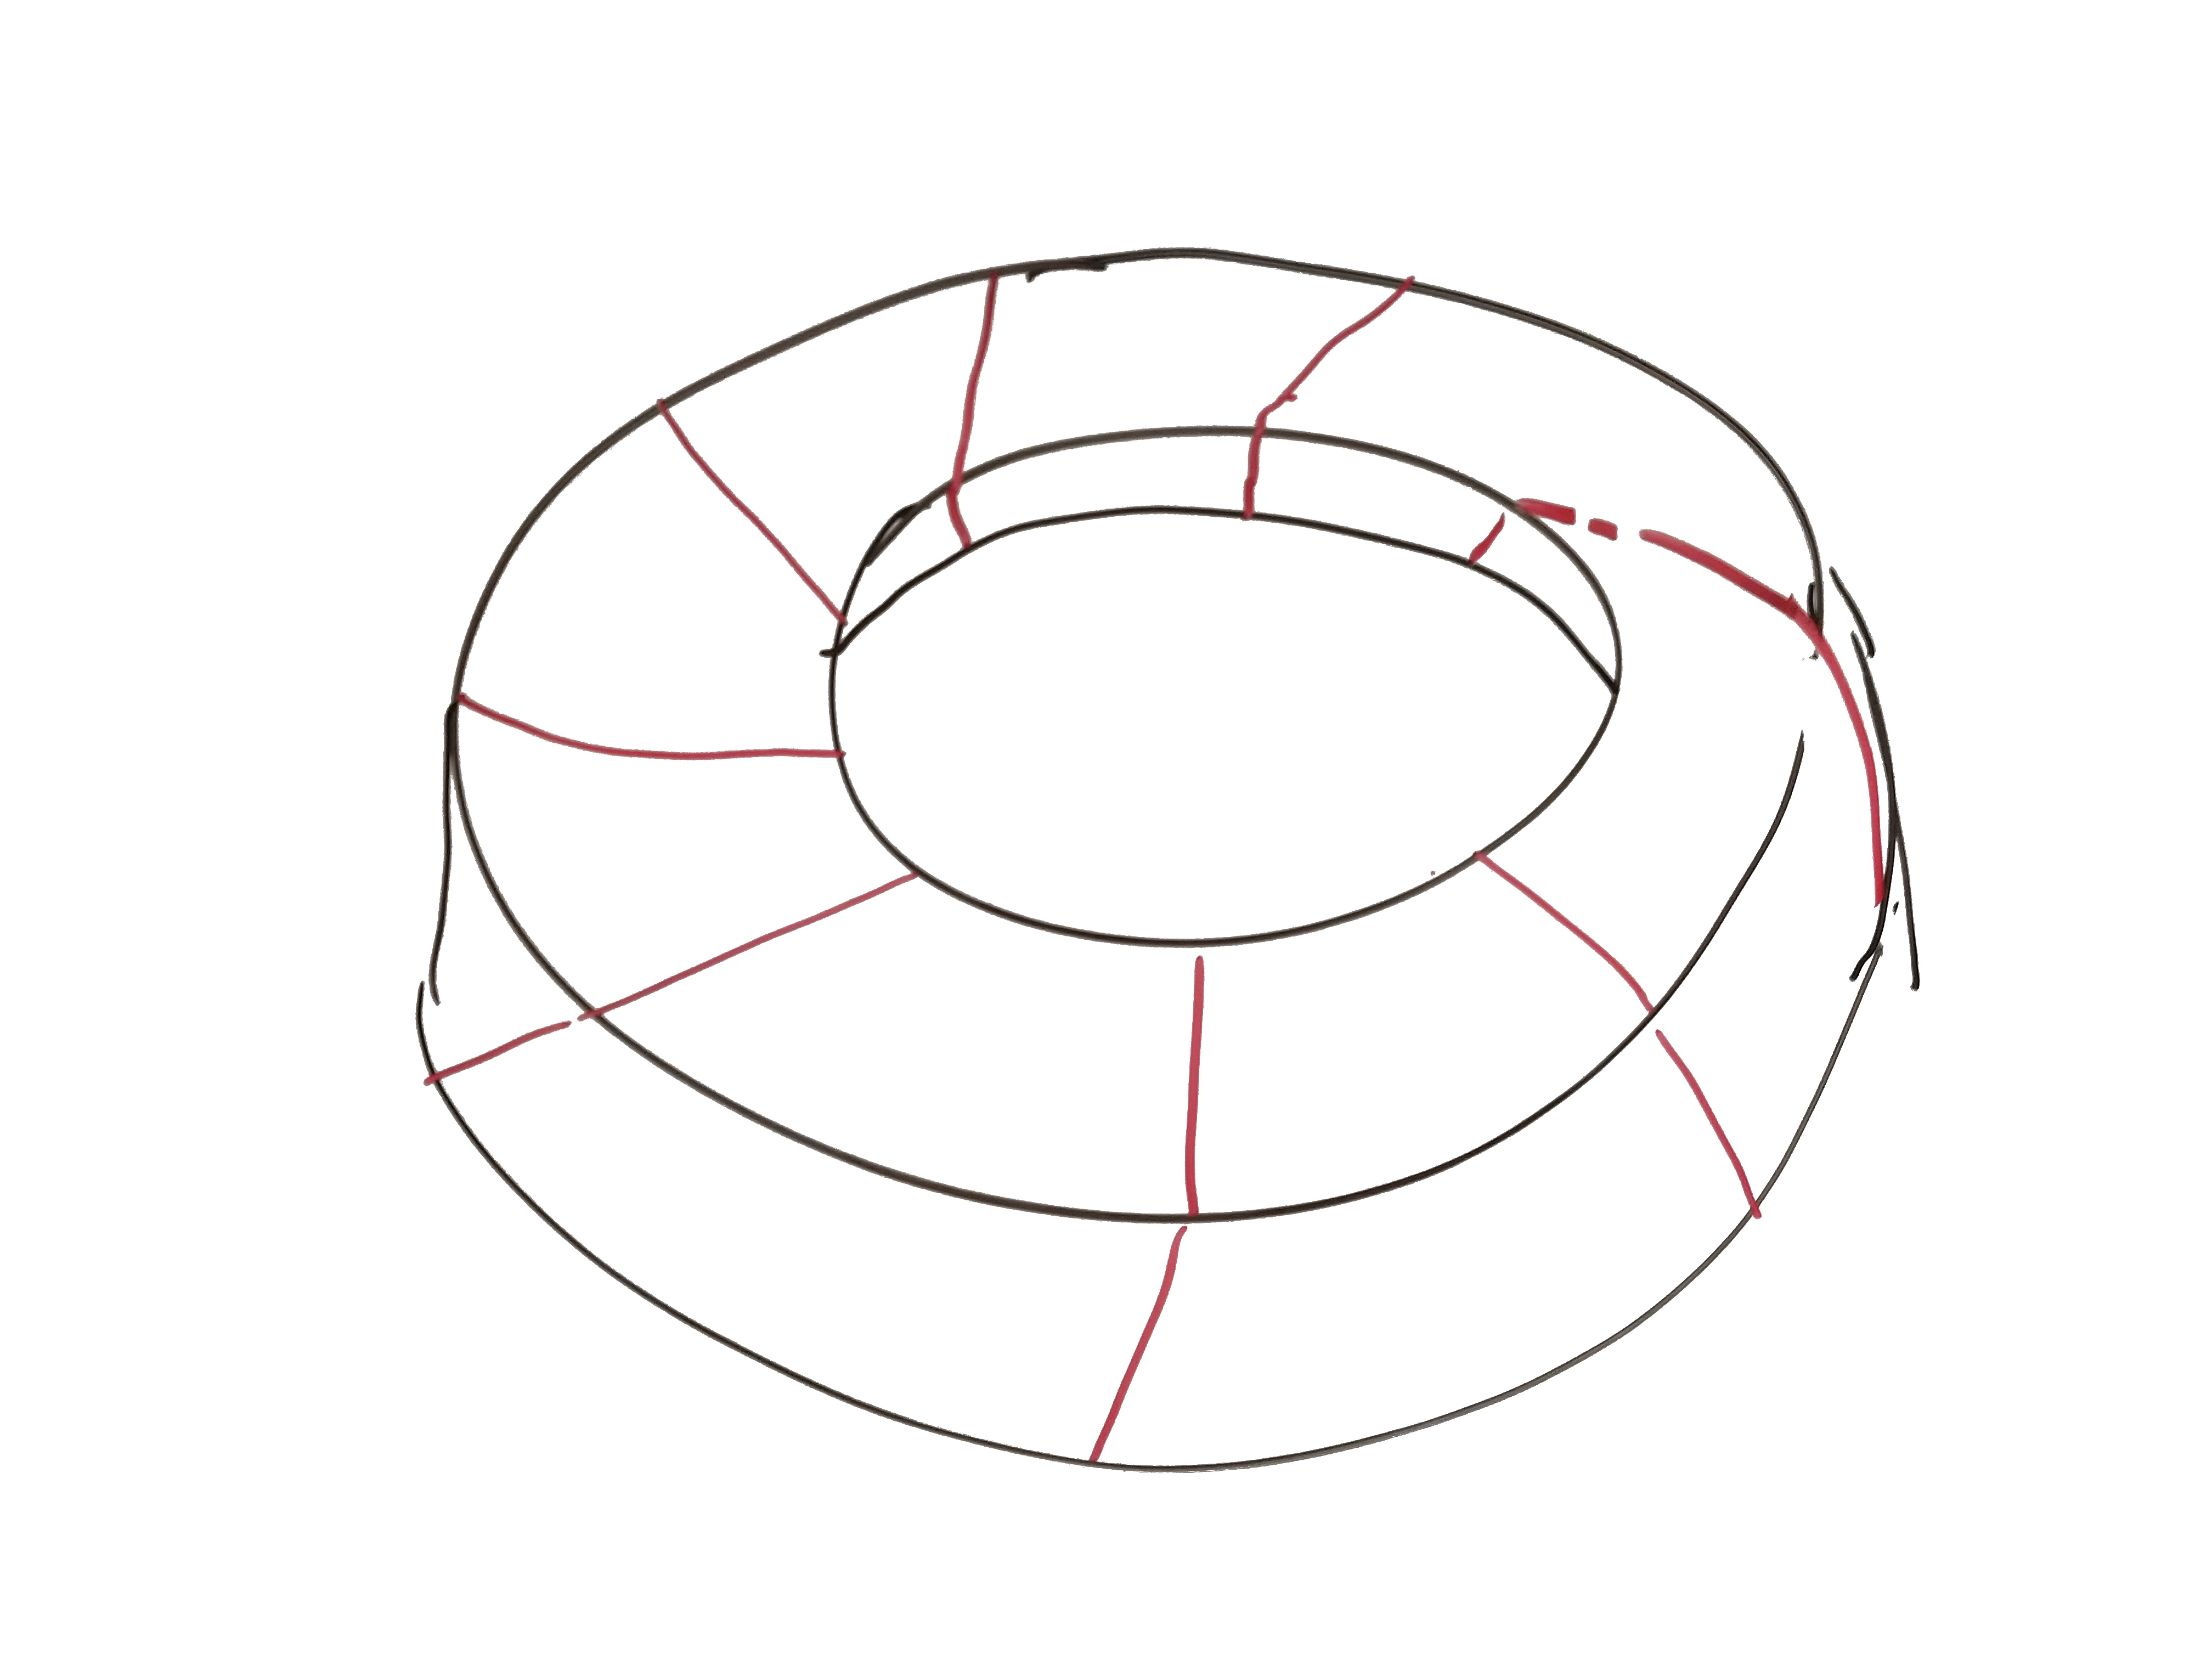
\includegraphics[width=6cm]{1_1.jpg}
		\caption{Nicht idealisierte Toroidspule}
	\end{subfigure}
	\quad
	\begin{subfigure}[b]{0.3\textwidth}
		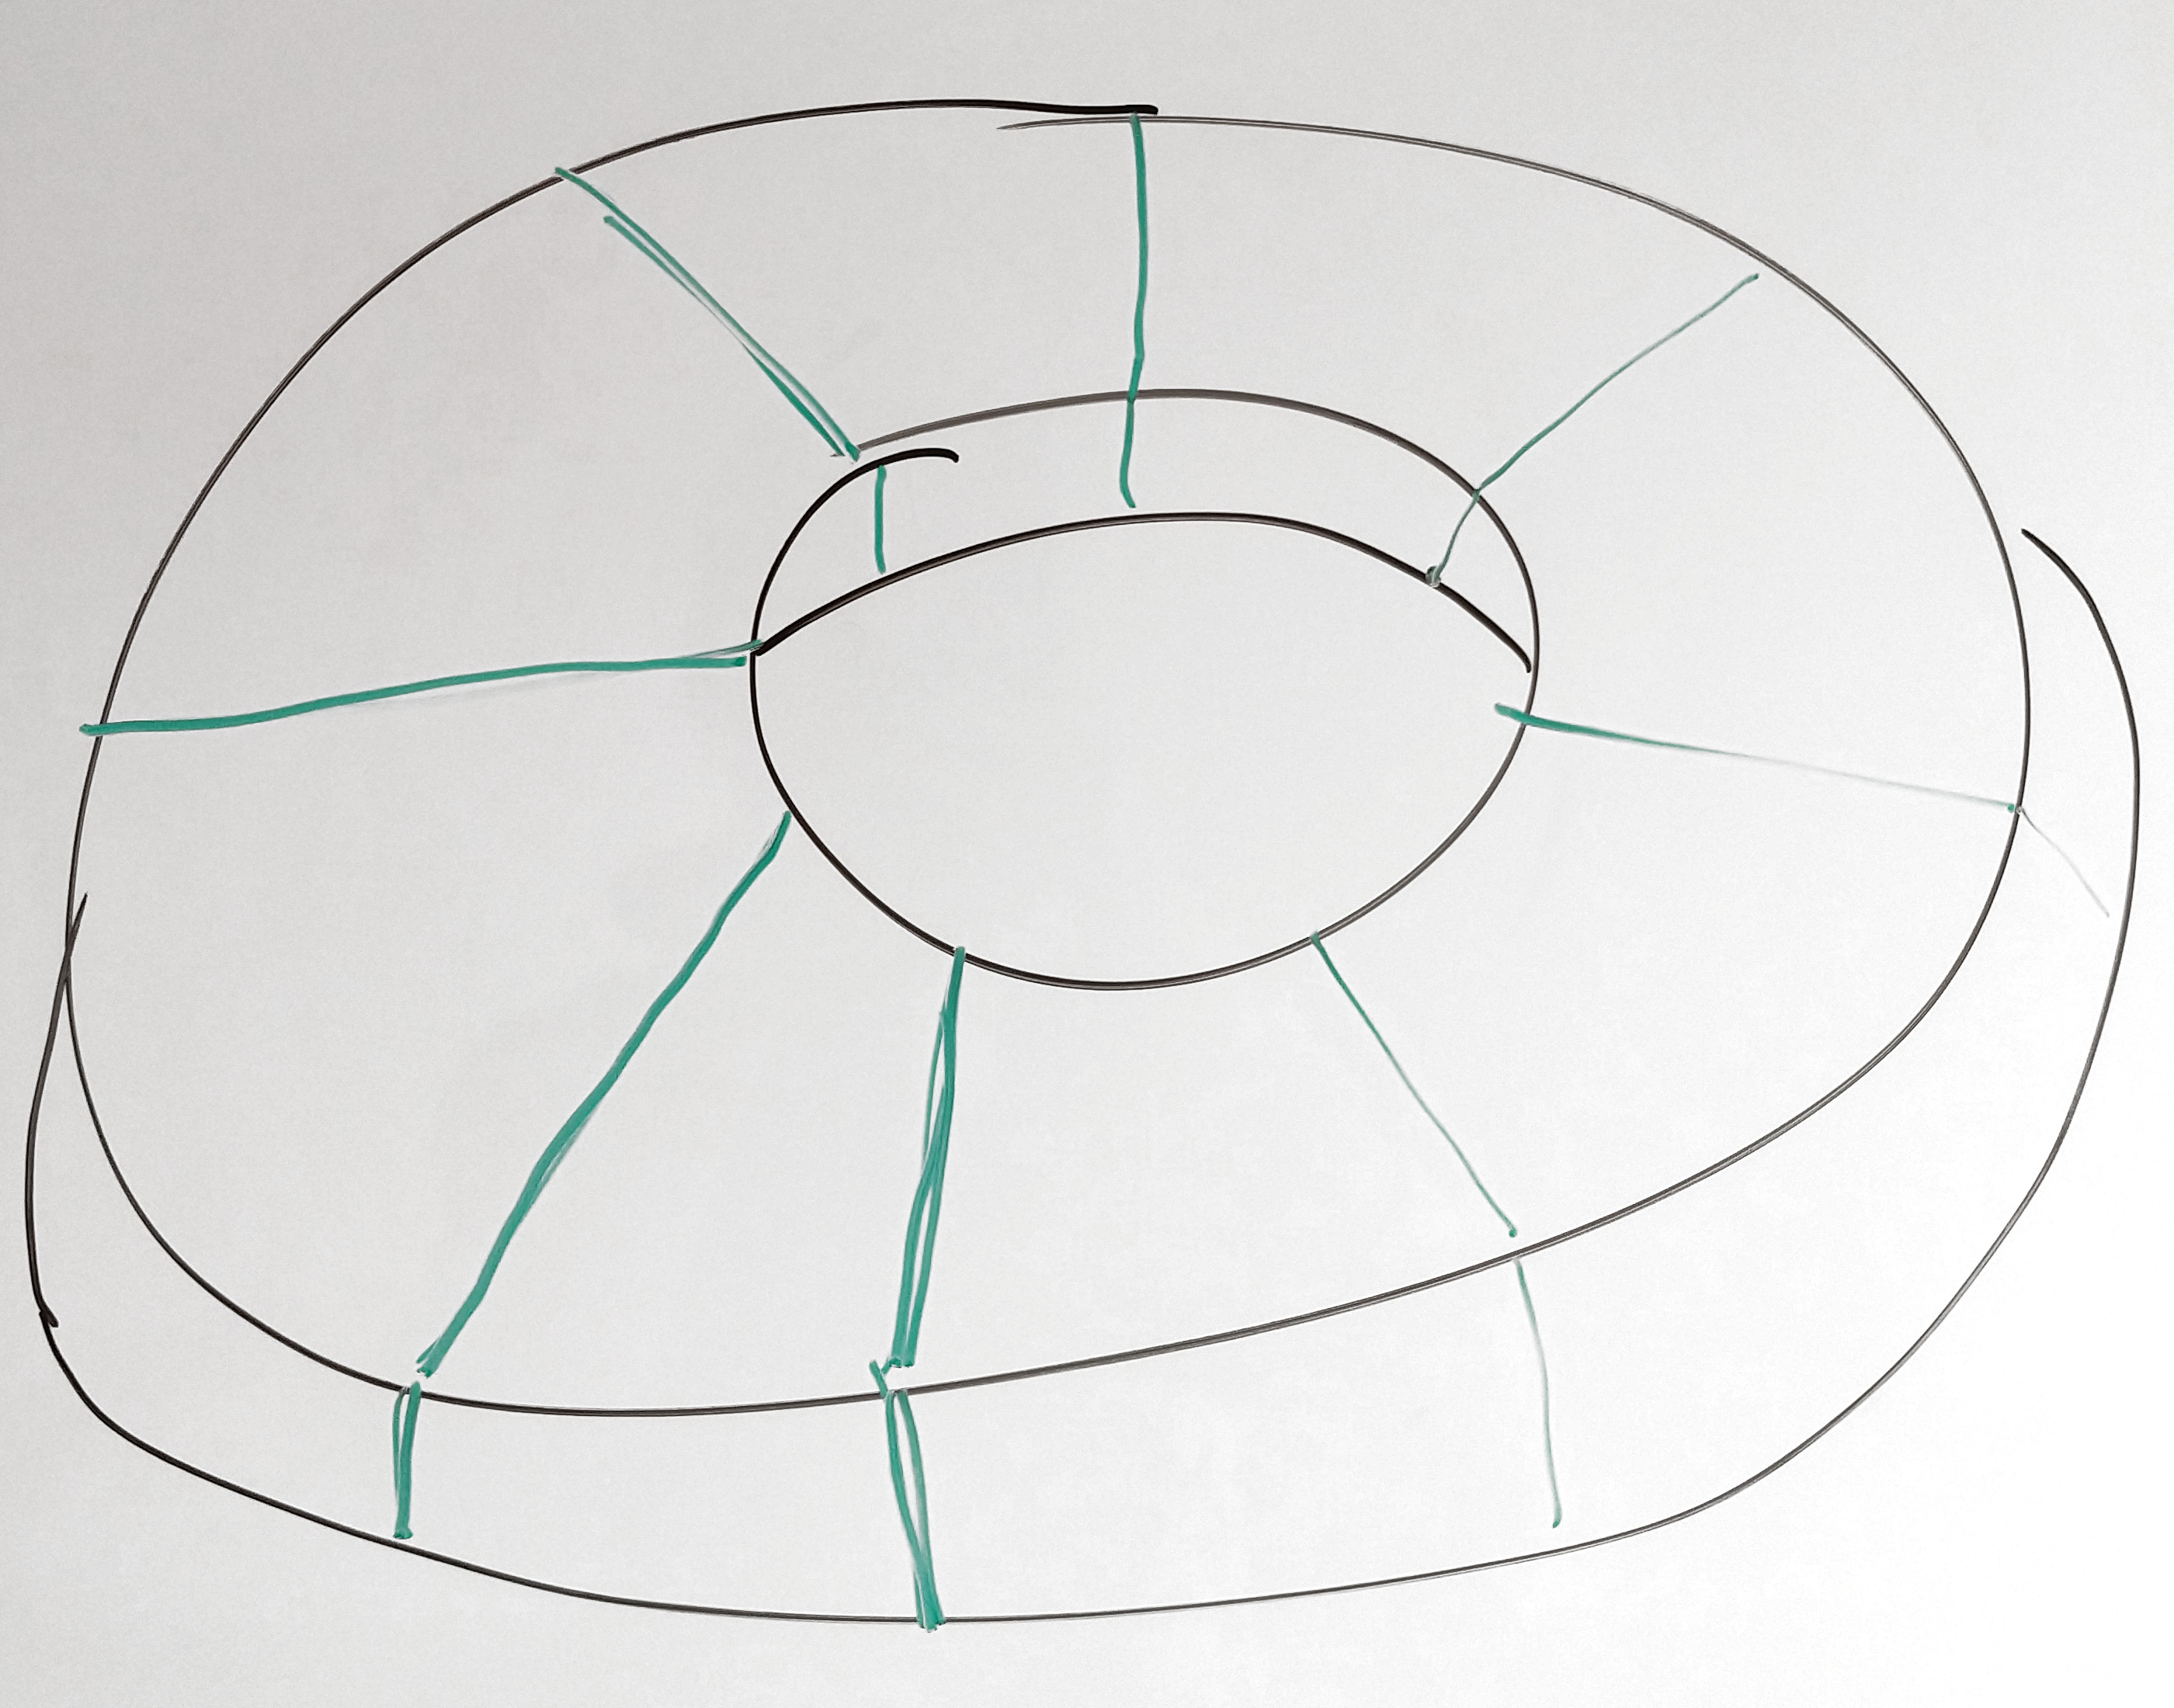
\includegraphics[width=6cm]{1_2.jpg}
		\caption{Idealisierte Toroidspule}
	\end{subfigure}
\end{figure}

b) Mit der Idealisierung, dass die einzelnen Windungen geschlossene
Leiterschleifen darstellen, erhalten wir das Feld im Inneren Bereich der 
Toroidspule mit dem Ampereschen Gesetz. \\
Der weg stellt dabei eine Umrundung im Torus dar. Aufgrund der Symmetrie
kann das $B$-Feld als annähernd konstant angenommen werden.\\
Die Fläche innerhalb dieser Umrundung wird natürlich $N$ mal vom Leiter
durchstoßen, d.h. $I_\text{enc} = NI$:
\begin{align*}
	\text{Amperesches Gesetz } \oint \mathbf B \cdot d\mathbf l &=
	\mu_0 I_\text{enc} \\
	\Rightarrow
	B_i \cdot l 	&= \mu_0 I_\text{enc} \\
			&= \mu_0 NI \\
	% umstellen
	B_i(r) 		&= \frac{\mu_0 NI}{2\pi r}
\end{align*}

c) Der Magnetische Fluß folgt aus dem Ergebniss aus b):
\begin{align*}
	\phi &= \iint \vec B \cdot d\vec A \\
	% flaeche parametrisieren
	&= \int_0^h \int_{R_1}^{R_2} B(r) \ dr dz \\
	% z integrieren, b einsetzne
	&= h \cdot \int_{R_1}^{R_2} \frac{\mu_0 NI}{2\pi r} dr \\
	% r integrieren
	&= h \cdot \frac{\mu_0 NI}{2\pi} \ln\left(\
		\frac{R_2}{R_1} \right)
\end{align*}


\newpage
\setlength{\headheight}{0cm}
\section*{Aufgabe 2}
Biot-Savar'sches Gesetz:
\[
	\mathbf B(\mathbf r) = \frac{\mu_0}{4\pi} I \int \frac
	{d\mathbf l \times (\mathbf r - \mathbf{r^\prime})}
	{\vert \mathbf r - \mathbf{r^\prime}\vert^3}
\]
Zur einfacheren Berechnung teilen wir den Draht in die zwei geraden 
Segmente (welche aufgrund der Symmetrie das Gleiche Feld am Punkt $P$ 
besitzen) und in das Halbkreissegment auf. \\
Zur Verinfachung wird das Koordinatensystem so gelegt, dass der Punkt 
$P$ im Urspung liegt. 
\newline
Berechnung des Halbkreissegements:
\begin{align*}
	\mathbf B_{HK}(\mathbf r) 
	&= \frac{\mu_0}{4\pi} I \int \frac
	{d\mathbf l \times (\mathbf r - \mathbf{r^\prime})}
	{\vert \mathbf r - \mathbf{r^\prime}\vert^3} \\
	% parametrisierung und zylinder koordianten
	&= \frac{\mu_0}{4\pi} I
	\int_0^\infty \int_{-\infty}^\infty \int_0^{2\pi}
	\frac
	{\vec e_\varphi \times (\mathbf r - \mathbf{r^\prime})}
	{\vert \mathbf r - \mathbf{r^\prime}\vert^3}
	\cdot r^\prime \cdot
	\delta(z^\prime) \cdot \delta(r^\prime - R) \cdot 
	\Theta(\pi - \varphi^\prime)
	\ d\varphi^\prime dz^\prime d\rho^\prime \\
	% r = ursprung
	&= \frac{\mu_0}{4\pi} I
	\int_0^{\pi}
	\frac
	{\vec e_\varphi \times \mathbf{r^\prime}}
	{\vert \mathbf{r^\prime}\vert^3} \cdot R
	\ d\varphi^\prime \\
	% kuerzen
	&= \frac{\mu_0}{4\pi} I
	\int_0^{\pi} \frac
	{\vec e_\varphi \times \vec e_\rho}
	{R^2}
	\cdot R
	\ d\varphi^\prime \\
	% kreuzprodukt ausrechnen
	&= \frac{\mu_0}{4\pi} I
	\int_0^{\pi} \frac
	{\vec e_z}
	{R}
	\ d\varphi^\prime \\
	% integrieren und kuerzen
	&= \frac{\mu_0 \ I}{4R} \vec e_z
\end{align*}
Die Berechnung des geraden Leiterelements erfolgt mit der Formel für das
Magnetfeld des endlichen Leiters, in Abhängigkeit von den  Winkeln an den 
Enden:
\begin{align*}
	B_{ger} (\mathbf r)
	&= \frac{\mu_0 \ I}{4 \pi R} 
	(\sin \theta_2 - \sin \theta_1) \\
	% winkel einsetzen
	&= \frac{\mu_0 \ I}{4 \pi R} 
	\left( \sin \frac\pi2 - \sin 0 \right) \\
	% ausrechnen
	&= \frac{\mu_0 \ I}{4\pi R}
\end{align*}
Das Magnetfeld folgt dann:
\[
	\mathbf B(\mathbf r) = \mathbf B_{HK}(\mathbf r) +
	2 \ \mathbf B_{ger} (\mathbf r)
	= \frac{\mu_0 \ I}{4R} \vec e_z + \frac{\mu_0 \ I}{2\pi R} \vec e_z
	= \frac{\pi + 2}{4\pi R} \mu_0 \ I \ \vec e_z
	\]

\newpage
\setlength{\headheight}{0cm}
\section*{Aufgabe 3}
Das magnetische Feld kann mit dem Biot-Savart Gesetz ermittelt werden:
\begin{align*}
	\mathbf B(\mathbf r) 
	&= \frac{\mu_0}{4\pi} \cdot I \cdot \int 
	\frac{d \mathbf{l} \times (\mathbf{r} - \mathbf{r^\prime})}
	{\vert \mathbf{r} - \mathbf{r^\prime} \vert^3} \\
	% parametrisierung des leiters
	&= \frac{\mu_0}{4\pi} \cdot I \cdot 
	\int_0^\infty \int_{-\infty}^\infty \int_0^{2\pi}
	\frac{\vec e_\varphi \times 
	(\mathbf{r} - \mathbf{r^\prime})}
	{\vert \mathbf{r} - \mathbf{r^\prime} \vert^3} \cdot
	\delta(R - \rho^\prime) \cdot \delta(z^\prime) \cdot \rho^\prime
	\ d\rho^\prime \ dz^\prime \ d\varphi^\prime \\
	% delta funktionen integrieren
	&= \frac{\mu_0}{4\pi} \cdot I \cdot 
	\int_0^{2\pi}
	\frac{ \vec e_\varphi \times 
	(z \ \vec e_z - r^\prime \vec e_\rho)}
	{\left( R^2 + z^2 \right)^{1.5} } \cdot
	R
	\ d\varphi^\prime \\
	% kreuzprodukte ermitteln
	&= \frac{\mu_0}{4\pi} \cdot I \cdot 
	\int_0^{2\pi}
	\frac{z \ \vec e_\rho + R \ \vec e_z}
	{\left( R^2 + z^2 \right)^{1.5} } \cdot
	R
	\ d\varphi^\prime
\end{align*}
Da sich der Magnetische Dipol auf der $z$-Achse befindet, verschwindet der
$\vec e_\rho$.
\begin{align*}
	\Rightarrow
	\mathbf B(\mathbf r) 
	&= \frac{\mu_0}{4\pi} \cdot I \cdot 
	\int_0^{2\pi}
	\frac{R^2 \ \vec e_z}
	{\left( R^2 + z^2 \right)^{1.5} }
	\ d\varphi^\prime \\
	% nach phi integrieren
	&= \frac{\mu_0 \ I}{2}
	\frac{R^2 \ \vec e_z}
	{\left( R^2 + z^2 \right)^{1.5} }
\end{align*}
Daraus folgt die Kraft auf ein magnetisches Dipol $m$:
\begin{align*}
	\mathbf F 
	&= m_z \ \partial_z B_z \ \vec e_z \\
	% einsetzen
	&= m_z \ 
	\frac{R^2 \ \mu_0 \ I}{2}
	\ \partial_z 
	\left( R^2 + z^2 \right)^{-1.5}
	\vec e_z \\
	% ableiten
	&= m_z \ 
	\frac{R^2 \ \mu_0 \ I}{2}
	\ (-1.5)
	\left( R^2 + z^2 \right)^{-2.5} \cdot 2z \
	\vec e_z \\
	% bisschen ordentlicher hinschreiben
	&= \frac{-1.5 z \cdot m_z \ R^2 \ \mu_0 \ I}
	{(R^2 + z^2)^{2.5}} \ \vec e_z
\end{align*}
Für kleine Auslenkungen, also $z \ll R$ vereinfacht sich die Kraft:
\begin{align*}
	z \ll R \Rightarrow R^2 + z^2 \approx R^2 \Rightarrow
	\mathbf F
	&= \frac{-1.5 z \cdot m_z \ R^2 \ \mu_0 \ I}
	{R^5} \ \vec e_z \\
	% kuerzen
	&= \frac{-1.5 z \cdot m_z \ \mu_0 \ I}
	{R^3} \ \vec e_z
\end{align*}
Schreibt man diesen Ausdruck als Differentialgleichung erhalten wir den
harmonischen Oszillator:
\begin{align*}
	F_z = M\ddot z 
	&= \frac{-1.5 z \cdot m_z \ \mu_0 \ I}
	{R^3} \Rightarrow
	\ddot z + \underbrace{\frac{1.5\cdot m_z \ \mu_0 \ I}{M \cdot R^3}}
	_{\omega^2} \ z = 0
\end{align*}
Mit der uns schon bekannten Lösung:
\[
	z(t) = z(0) \cos(\omega t) + \dot z(0) \sin(\omega t)
\]

\newpage
\section*{Aufgabe 4}
\[
	\vec B(\vec r) = B \vec e_z, \ B = const. \tag{4.1}
\]
a) gesucht sei ein $\vec A$, sodass
\[ \rot \vec A = \vec B \]

Mit dem Ansatz 
\[
	\vec A = M \cdot \vec r, \quad
	\vec r = (x,y,z)^T, \
	M \in \mathbb{R}^{3\times3}
\]

sind die Einträge von $M$ die partiellen Ableitungen von $\vec A$:
\[ M_{ij} = \partial_j A_i \tag{4.2} \]

Aus der Vorraussetzung $\rot \vec A =\vec B$ folgen die Bedinungen für 
$M$:
\begin{align*}
	\rot \vec A = \begin{pmatrix}
		M_{3,2} - M_{2,3} \\
		M_{1,3} - M_{3,1} \\
		M_{2,1} - M_{1,2} 
	\end{pmatrix}
	\overset{!}{=}
	\begin{pmatrix} 0 \\ 0 \\ B \end{pmatrix}
	\ \Rightarrow \
	M_{3,2} = M_{2,3}, \
	M_{1,3} = M_{3,1}, \
	M_{2,1} = M_{1,2} +B
	\tag{4.3}
\end{align*}

Daraus folgt dann die Matrix $M$ (mit den Freiheitsgraden $\alpha$, ...):
\[
	M = \begin{pmatrix}
		\alpha 		&\beta 		&\gamma \\
		\beta + B 	&\delta 	&\epsilon \\
		\gamma 		&\epsilon 	&\zeta
	\end{pmatrix}
\]

Das einfachste Vektorfeld für $\vec A$ wäre das wo alle Freiheitsgrade auf 
0 gesetzt werden:
\[
	\vec A_0 = M_0 \cdot \vec r = 
	M = \begin{pmatrix}
		0 &0 &0 \\ \beta &0 &0 \\ 0 &0 &0
	\end{pmatrix}
	\cdot \begin{pmatrix}
		x \\ y \\ z
	\end{pmatrix}
	= 
	\begin{pmatrix}
		0 \\ Bx \\0
	\end{pmatrix}
\]
\vspace{0.5cm}
b) $A_1$ und $A_2$ seien zwei linear unabhängige Lösungen von (4.1). Dann 
lässt sich für eine Linearkombination 
\begin{align*}
	\vec A^\prime = \alpha_1 \vec A_1 + \alpha_2 \vec A_2
	\quad \text{(mit $\alpha_1 + \alpha_2 = 1$)}
\end{align*}

zeigen:
\begin{align*}
	\vec \nabla \times \vec A^\prime
	&= \vec \nabla \times \left(
		\alpha_1 \vec A_1 + \alpha_2 \vec A_2
	\right) \\
	% matrix einsetzen
	&= \vec \nabla \times \left(
		\alpha_1 M_1 \cdot \vec r + \alpha_2 M_2 \cdot \vec r
	\right) \\
	% kommutativgesetz
	&= \vec \nabla \times \left(
		(\alpha_1 M_1 + \alpha_2 M_2) \cdot \vec r
	\right) \\
	% indexnotation beim matrix produkt
	&= \vec \nabla \times \left(
		\sum_{i j} x_i (\alpha_1 \ M_{1, ij} + 
		\alpha_2 \ M_{2, ij})
	\right) \\ 
	% kreuzprodukt mit epsilon tensor
	&= \sum_{m n i j} \epsilon_{mni} \  \underbrace{\partial_{x_n} x_i 
	(\alpha_1 \ M_{1, ij} + \alpha_2 \ M_{2, ij})}_{
		(4.2) \Rightarrow \ =\alpha_1 M_{1, in} 
		+ \alpha_2 M_{2, in}}
	\cdot \hat x_m \\[0.1cm]
	% 4.2 anwenden
	&= \sum_{m n i} \epsilon_{mni} \
		\left( \alpha_1 M_{1, in} + \alpha_2 M_{2, in} \right)
	\cdot \hat x_m \\
	% 4.3 anwenden
	(4.3) \Rightarrow \ 
	&= \sum_{n i} \epsilon_{3ni} \
		\left( \alpha_1 M_{1, in} + \alpha_2 M_{2, in} \right)
	\cdot \hat x_3 \\
	% indizes einsetzen
	&= \left( \alpha_1 (M_{1,21} - M_{1,12}) + \alpha_2
		(M_{2,21} - M_{2,12}) \right) \vec e_z \\
	% 4.3 anwenden
	(4.3) \Rightarrow \ 
	&= \left( \alpha_1 B + \alpha_2 B \right) \vec e_z \\
	% b rausziehen
	&= \left( \alpha_1 + \alpha_2 \right) B \vec e_z \\
	&= B \vec e_z
\end{align*}
\newpage
c)
\begin{align*}
	\vec\nabla \times \vec A^{\prime\prime} 
	&= \vec\nabla \times (\vec A + \vec\nabla \phi) \\
	&= \vec\nabla \times \vec A + 
	\underbrace{\vec\nabla \times (\vec\nabla \phi)}_{=0} \\
	&= \vec B
\end{align*}
\vspace{0.5cm}
d)
Die Differenz lässt sich auch umschreiben:
\[
	\vec A^\prime - \vec A 
	= M^\prime \cdot \vec r - M \cot r
	= (M^\prime - M) \cdot r
\]
Für diese Differenzmatrix $D := M^\prime - M$ können wir bestimmen:
\[
	D_{21} = M_{21}^\prime - M_{21} 
	= M_{12}^\prime + B - M_{12} - B = M_{12}^\prime - M_{12}
\]
da sich die Differenz bei $M_{21}$ und $M_{12}$ jetzt auslöscht, 
kann man für die Differenzmatrix $D := M^\prime - M$ schreiben:
\[
	D_{ij} = D_{ji} \text{ für alle } j,i.
\]
Damit extistiert ein ``Differenzfeld``:
\[
	\vec d := D \cdot r =
	\begin{pmatrix}
		D_{11} \cdot x + D_{12} \cdot y + D_{13} \cdot z \\
		D_{12} \cdot x + D_{22} \cdot y + D_{23} \cdot z \\
		D_{13} \cdot x + D_{23} \cdot y + D_{33} \cdot z
	\end{pmatrix}
\]
Zu diesem Feld existiert immer ein Potential U:
\begin{align*}
	U &= \int d_x \ dx =
	\frac{D_{11}}2 \cdot x^2 + D_{12} \cdot yx + D_{13} \cdot zx + C_1 
\\
	U &= \int d_y \ dy =
	D_{12} \cdot xy + \frac{D_{22}}2 \cdot y^2 + D_{23} \cdot zy + C_2
\\
	U &= \int d_z \ dz =
	D_{13} \cdot xz + D_{23} \cdot yz + \frac{D_{33}}2 \cdot z^2 + C_3
\\
\Rightarrow
	U &= \frac{D_{11}}2 \cdot x^2 + \frac{D_{22}}2 \cdot y^2 
	+ \frac{D_{33}}2 \cdot z^2 + D_{12} \cdot yx + D_{13} \cdot zx
	+ D_{23} \cdot yz
\end{align*}
\vspace{0.5cm}
e) Die Eichfreiheit beim Vektorpotential gibt Möglichkeiten für 
Randbedinungen beim berechnen.
\begin{figure}[H]
	\centering
	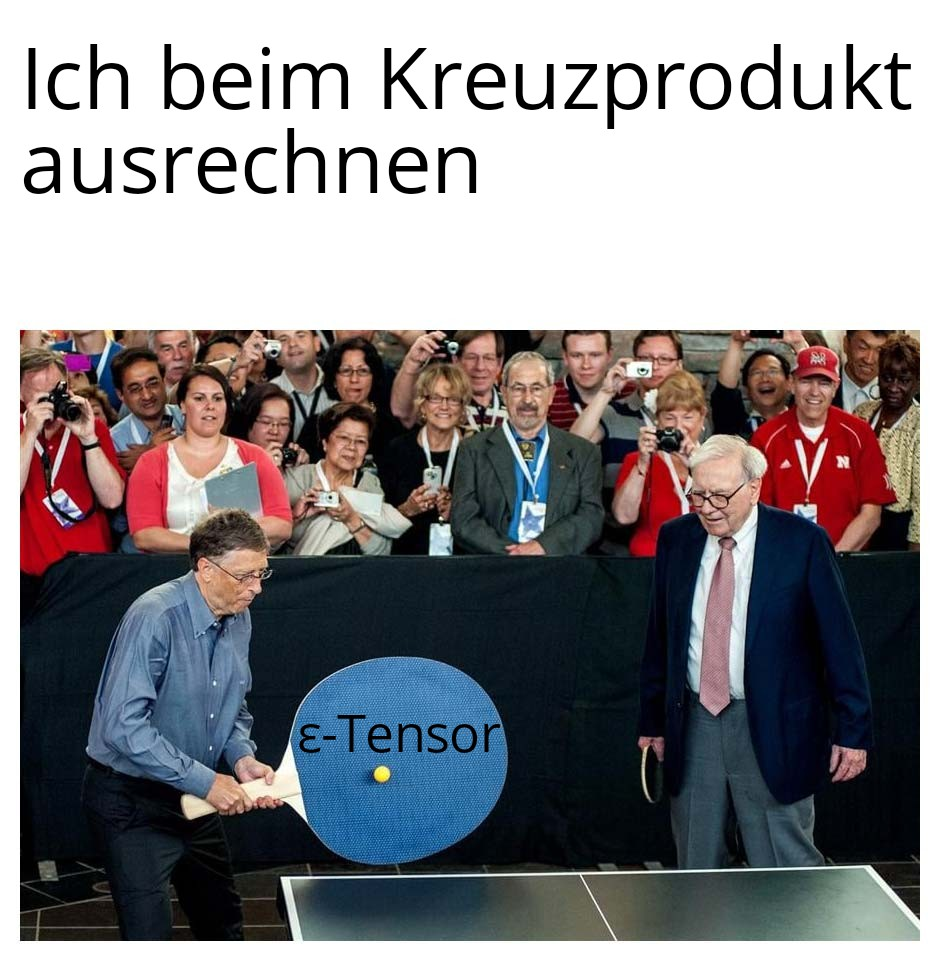
\includegraphics[width=7cm]{aufgabe4_meme.jpg}
\end{figure}

\newpage
\section*{Aufgabe 5}
Wir können die geknickte Fläche aufteilen in zwei flache Leiterschleifen, 
wo das Dipolmoment gegeben ist durch
\[ \vec m = I \cdot A \cdot \hat n. \]
Das kombinierte Dipolmoment entspricht dann der vektoriellen Summe
\[
	\vec m = \vec m_1 + \vec m_2 
	= Iw^2 \vec e_z + Iw^2 \vec e_z
\]
Entlang der $x$-Achse verlaufen die zwei Ströme gegenläufig, sodass der 
Gesamtstrom an der Stelle 0 ist (ensprechend der Randbedingung).
\begin{figure}[H]
	\centering
	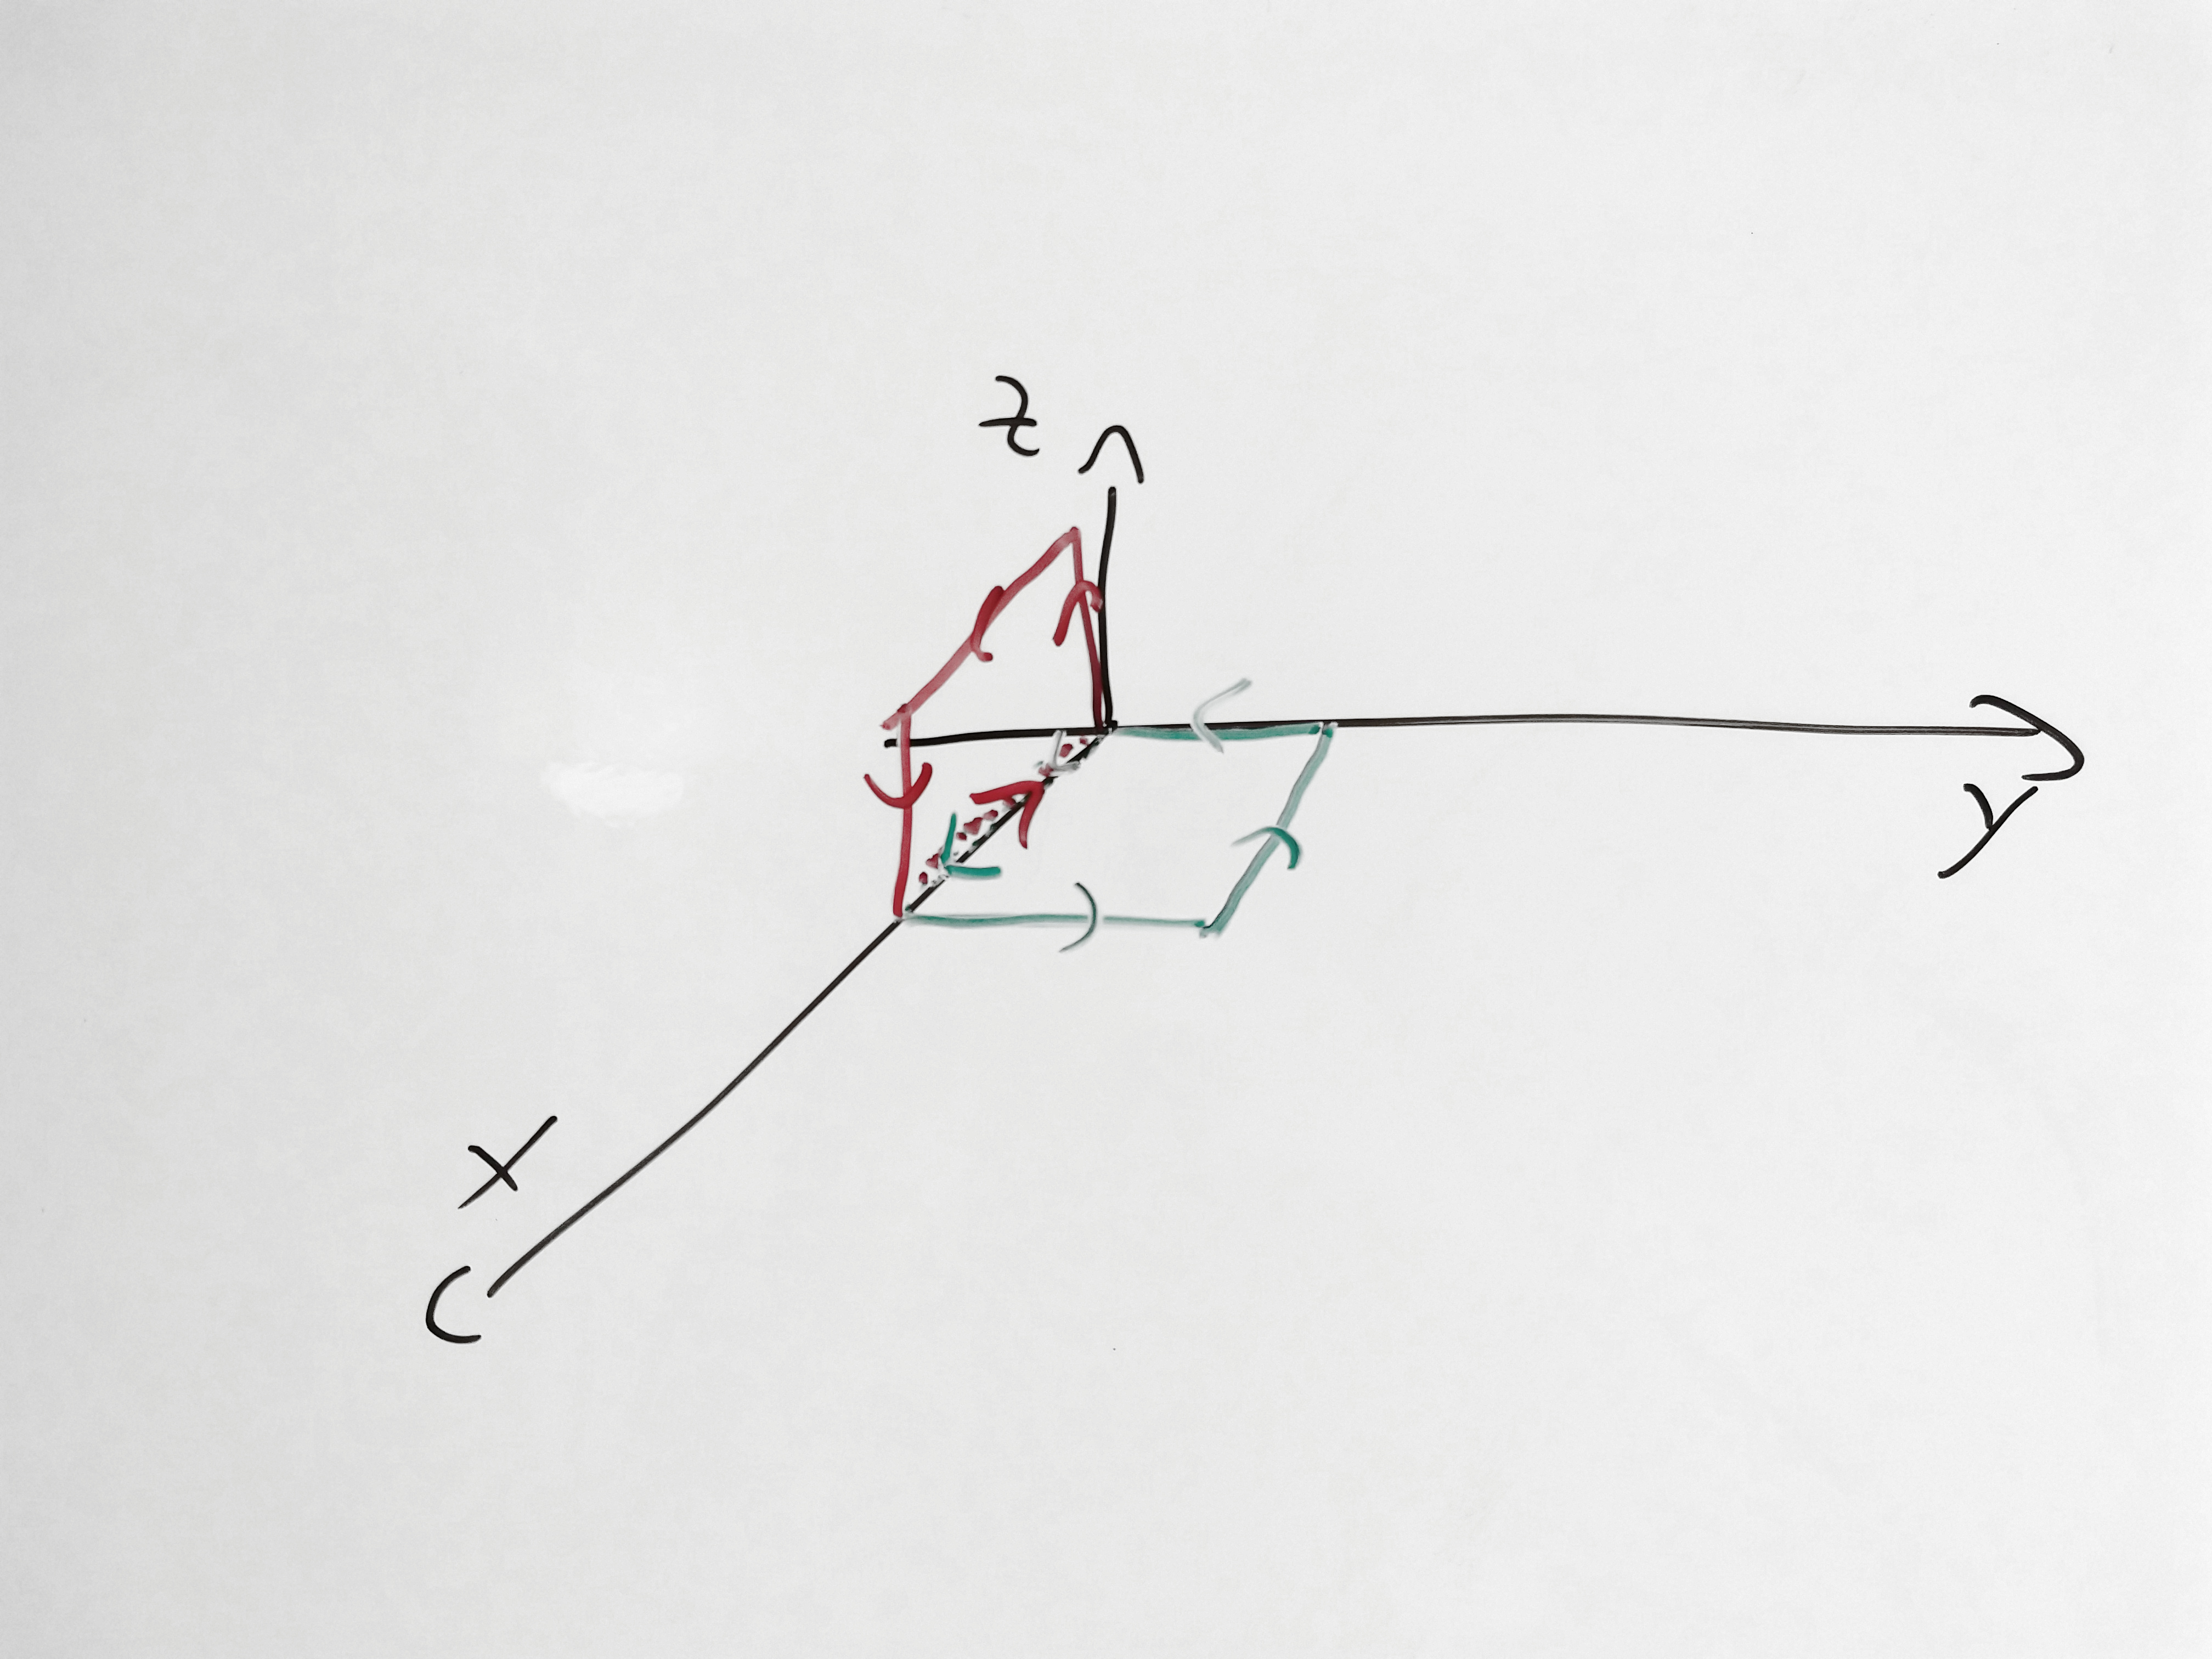
\includegraphics[width=10cm]{5_1}
	\caption{Aufteilung in zwei Schleifen}
\end{figure}

\end{document}
